%%%%%%%%%%%%%%%%%%%%%%%%%%%%%%%%%%%%%%%%%
% Beamer Presentation
% LaTeX Template
% Version 1.0 (10/11/12)
%
% This template has been downloaded from:
% http://www.LaTeXTemplates.com
%
% License:
% CC BY-NC-SA 3.0 (http://creativecommons.org/licenses/by-nc-sa/3.0/)
%
%%%%%%%%%%%%%%%%%%%%%%%%%%%%%%%%%%%%%%%%%

%----------------------------------------------------------------------------------------
%	PACKAGES AND THEMES
%----------------------------------------------------------------------------------------

\documentclass{beamer}

\mode<presentation> {

% The Beamer class comes with a number of default slide themes
% which change the colors and layouts of slides. Below this is a list
% of all the themes, uncomment each in turn to see what they look like.

%\usetheme{default}
%\usetheme{AnnArbor}
%\usetheme{Antibes}
%\usetheme{Bergen}
%\usetheme{Berkeley}
%\usetheme{Berlin}
%\usetheme{Boadilla}
%\usetheme{CambridgeUS}
%\usetheme{Copenhagen}
%\usetheme{Darmstadt}
%\usetheme{Dresden}
%\usetheme{Frankfurt}
%\usetheme{Goettingen}
%\usetheme{Hannover}
%\usetheme{Ilmenau}
%\usetheme{JuanLesPins}
%\usetheme{Luebeck}
\usetheme{Madrid}
%\usetheme{Malmoe}
%\usetheme{Marburg}
%\usetheme{Montpellier}
%\usetheme{PaloAlto}
%\usetheme{Pittsburgh}
%\usetheme{Rochester}
%\usetheme{Singapore}
%\usetheme{Szeged}
%\usetheme{Warsaw}

% As well as themes, the Beamer class has a number of color themes
% for any slide theme. Uncomment each of these in turn to see how it
% changes the colors of your current slide theme.

%\usecolortheme{albatross}
%\usecolortheme{beaver}
%\usecolortheme{beetle}
%\usecolortheme{crane}
%\usecolortheme{dolphin}
%\usecolortheme{dove}
%\usecolortheme{fly}
%\usecolortheme{lily}
%\usecolortheme{orchid}
%\usecolortheme{rose}
%\usecolortheme{seagull}
%\usecolortheme{seahorse}
%\usecolortheme{whale}
%\usecolortheme{wolverine}

%\setbeamertemplate{footline} % To remove the footer line in all slides uncomment this line
%\setbeamertemplate{footline}[page number] % To replace the footer line in all slides with a simple slide count uncomment this line

%\setbeamertemplate{navigation symbols}{} % To remove the navigation symbols from the bottom of all slides uncomment this line
}

\usepackage{graphicx} % Allows including images
\usepackage{booktabs} % Allows the use of \toprule, \midrule and \bottomrule in tables

%----------------------------------------------------------------------------------------
%	TITLE PAGE
%----------------------------------------------------------------------------------------

\title[LNG 230/SPV 221 Language Acquisition]{Word Acquisition I} % The short title appears at the bottom of every slide, the full title is only on the title page

\author{Xiaomeng Ma} % Your name
\institute[Graduate Center, CUNY] % Your institution as it will appear on the bottom of every slide, may be shorthand to save space
{Graduate Center, CUNY \\ % Your institution for the title page
\medskip
\textit{xma3@gradcenter.cuny.edu} % Your email address
}
\date{September 24, 2018} % Date, can be changed to a custom date

\begin{document}

\begin{frame}
\titlepage % Print the title page as the first slide
\end{frame}


%----------------------------------------------------------------------------------------
%	PRESENTATION SLIDES
%----------------------------------------------------------------------------------------

%------------------------------------------------
\section{First Section} % Sections can be created in order to organize your presentation into discrete blocks, all sections and subsections are automatically printed in the table of contents as an overview of the talk
%------------------------------------------------

\subsection{Subsection Example} % A subsection can be created just before a set of slides with a common theme to further break down your presentation into chunks

\begin{frame}{Introduction}
\begin{itemize}
\item How do we acquire the meaning of a word? 
\pause 
\item Infants and toddlers have amazing ability to learn words
\begin{itemize}
    \item Children as young as 12 month old already understand 50 words (Fenson et al., 1994)
    \item Children are able to learn words through fast mapping. 
    \\ "red tray, blue tray, chromium tray" (Carey and Bartlett (1978))
\end{itemize}

\end{itemize}
\end{frame}
%------------------------------------------------
\begin{frame}
\frametitle{Problems in Word Acquisition}
\begin{itemize}
\item Reference: The Gavagai problem
\\ https://www.youtube.com/watch?v=0YY4qxkqm3o 
\begin{itemize}
    \item  “With each referential act, e.g., ‘Look, a dog!’ there are an infinite number of hypotheses for the meaning of the word ‘dog’ that are consistent with the data” (Xu & Tenenbaum,2005,p.1).
    \pause
    \item What about abstract words, like "love",or "the"?
\end{itemize}
\end{itemize}
\end{frame}
%------------------------------------------------
\begin{frame}
\frametitle{Problems in Word Acquisition}
\begin{itemize}
\item Extension
\begin{figure}
    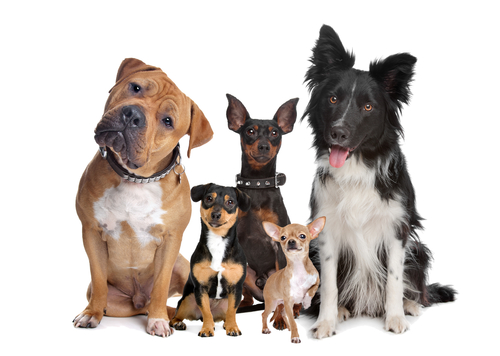
\includegraphics[height = 7cm, keepaspectratio]{diffeent-types-of-dog-breeds.jpg}
\end{figure}
\end{itemize}
\end{frame}
%------------------------------------------------
\begin{frame}
\frametitle{Problems in Word Acquisition}
\begin{itemize}
\item Extension
\begin{figure}
    
\includegraphics[height = 7cm, keepaspectratio]{57605685-cartoon-dog-faces-set-different-breeds-of-dogs-cute-flat-icons-.jpg}
\end{figure}
\end{itemize}
\end{frame}
%------------------------------------------------
\begin{frame}
\frametitle{Problems in Word Acquisition}
\begin{itemize}
\item Extension
\begin{figure}
    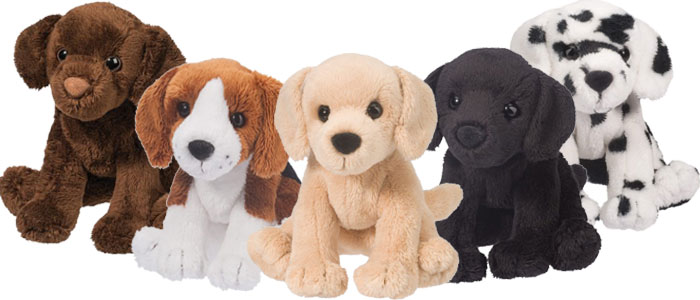
\includegraphics[wideth = \textwidth, keepaspectratio]{Douglas_MiniPups-1.jpg}
\end{figure}
\end{itemize}
\end{frame}
%------------------------------------------------
\begin{frame}
\frametitle{Problems in Word Acquisition}
\begin{itemize}
\item Extension 
\begin{itemize}
    \item Words are not always denote tangible things. They are used to denote categories/concepts. 
    \pause 
    \item Cross-linguistic difference
\end{itemize}
\end{itemize}
\end{frame}
%------------------------------------------------
\begin{frame}
\frametitle{Problems in Word Acquisition}
\begin{itemize}
\item Extension 
\begin{columns}
\begin{column}{0.45\textwidth}
\begin{figure}
    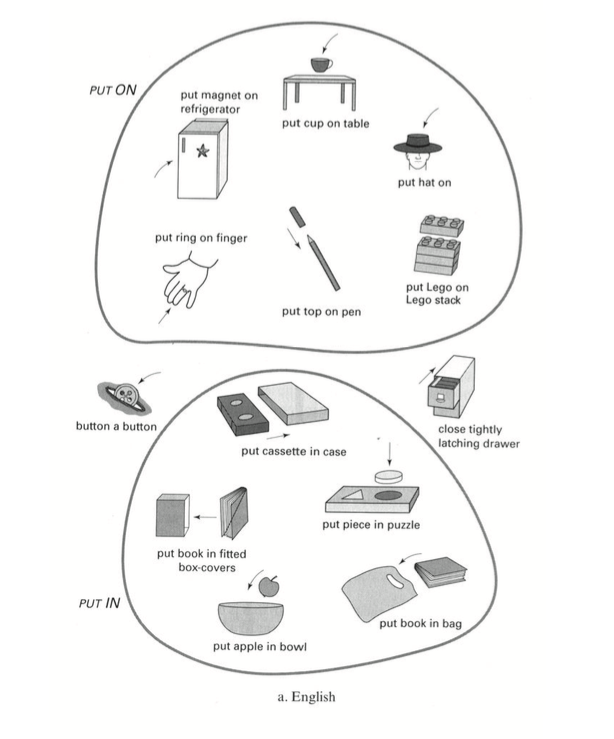
\includegraphics[height = 7cm, keepaspectratio]{english.png}
    \caption{English}
\end{figure}
\end{column}
\begin{column}{0.45\textwidth}
\begin{figure}
    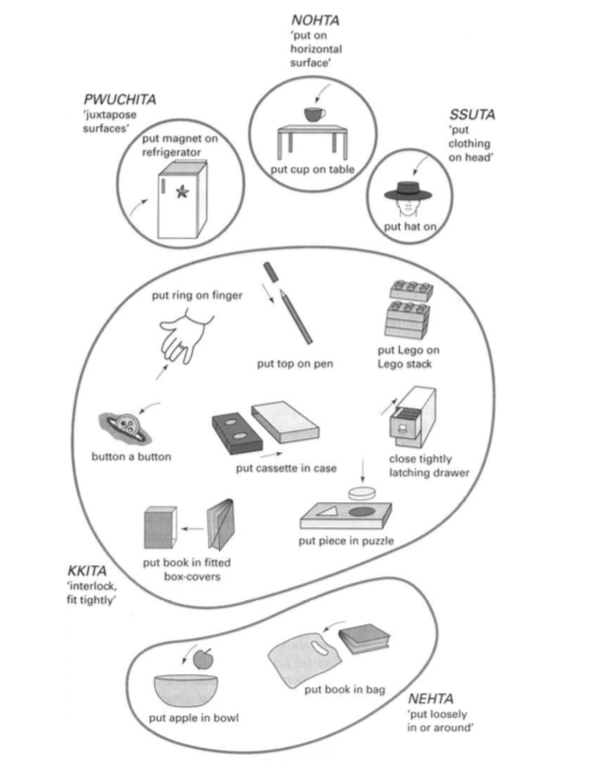
\includegraphics[height = 7cm, keepaspectratio]{korean.png}
    \caption{Korean}
\end{figure}
\end{column}
\end{columns}
\end{itemize}
\end{frame}
%------------------------------------------------
\begin{frame}
\frametitle{Problems in Word Acquisition}
\begin{itemize}
    \item Extension
    \begin{enumerate}
        \item Under-extension Errors: use words for a limited set of meanings
        \\ e.g \textit{up} and \textit{down} are used in motion event first, than extended to static and relations
        \pause
        \item Over-extension Errors: use words too broadly and in inappropriate ways
        \\ e.g \textit{open} --- pulling two Frisbees apart of pulling the stem off an apple
    \end{enumerate}
\end{itemize}
\end{frame}
%------------------------------------------------
\begin{frame}
\frametitle{Word Acquisition Summary}
\begin{itemize}
    \item Summary: To learn the meaning of a new word, the child not only has to isolate the correct referent for a word but also has to learn how to extend it appropriately for her language (while not over-extending it incorrectly)
    \pause
    \item HOW?
    \pause
    \item Not surprisingly, we don't know yet. But we have theories. 
\end{itemize}
\end{frame}
%------------------------------------------------
\begin{frame}
\frametitle{Constraints Theories}
\begin{itemize}
\item Claim: “children’s word learning is guided by a set of default assumptions or constraints on hypotheses” (Woodward & Markman, 1998, p. 379). 
\pause
\item Key Question: since new words can potentially refer to any aspect of an event, are we innately biased to consider some meanings before others?
\end{itemize}
\end{frame}

%------------------------------------------------
\begin{frame}
\frametitle{Constraints Theories}
\begin{itemize}
\item Whole item assumption: In the first instance, learners should assume that new words refer to whole objects, rather than parts of objects, actions, events or spatial relations. 
\\ e.g \textit{dog}: refers to whole dog, not dog's leg.
\pause
\item The mutual exclusivity assumption: Learners should assume that objects only have one name. 
\\ e.g \textit{dog running}: if we know that \textit{dog} refers to dog, then \textit{running} must mean something else. 
\pause
\item The taxonomic assumption: When learning how to extend a new word, assume that it will only extend to taxonomically related things, not thematically associated things.
\\ e.g \textit{dog}: can only extend to other dogs (cartoon dogs, stuffed dog toys), but not dog legs.
\item The shape bias: children to label objects of similar shapes with the same name.
\item The function bias: children to label novel objects that have the same function with the same name
\item Pragmatic principles of conventionality and contrast
\end{itemize}
\end{frame}
%------------------------------------------------
\begin{frame}
\frametitle{Evidence for the mutual exclusive assumption}
\textbc{Markman and Wachtel, 1988}
\begin{itemize}
\item Unfamiliar objects vs Familiar objects:
\begin{itemize}
    \item They showed the 3y/o picture of a cow and a radish rosette maker
    \item They asked the children to show them the \textit{mendel} (madeup word)
    \item The children chose raddish rosette maker over cow
\end{itemize}
\pause
\item Familiar object with unfamiliar label:
\begin{itemize}
    \item They showed the children a picture of fish and called the fish \textit{dorsal fin}
    \item They asked the children what is \textit{dorsal fin}, the whole fish or just the fin?
    \item The children chose the fin
\end{itemize}
\end{itemize}
\end{frame}
%------------------------------------------------
\begin{frame}
\frametitle{Evidence for the taxonomic assumption}
\textbc{Markman and Wachtel, 1984}
\begin{itemize}
    \item They showed 3y/o a cow and called it a \textit{dax}
    \item The children were divided into to groups:
    \\ Control group: Find another one.
    \\ Experiment group: Find another dax. (labelling)
    \item Objects included pig (taxonomic related) and milk (thematically related) and unrelated objects (car).
    \item The experiment group children are more likely to choose pig.
\end{itemize}
\end{frame}
%------------------------------------------------
\begin{frame}
\frametitle{Problems about these assumptions}
\begin{itemize}
\item What does the results really say about acquisition?
\pause 
\item If the constraints are innate, is it true for all languages?
\item Simply relying on constraints would point children in the wrong direction for a large number of words
\\ e.g Fido and dog
\end{itemize}
\end{frame}
%------------------------------------------------
\begin{frame}
\frametitle{Developmental Lexical Principles Framework }
\begin{itemize}
    \item First-tier (innate)
    \begin{itemize}
        \item The principle of reference. Children assume that words symbolise/stand for objects, actions and attributes.
        \item The principle of extendibility. Children assume that words do not necessarily refer to a single example  but to a category of similar objects.
        \item The principle of object scope. Children tend to assume a) that words refer to objects in the first place, and only apply labels to actions and events if it is clear that the word does not refer to an object and b) that words refer to the whole object not a part of the object.
    \end{itemize}
\end{itemize}
\end{frame}

%------------------------------------------------
\begin{frame}
\frametitle{Developmental Lexical Principles Framework }
\begin{itemize}
\item Second-tier 
    \begin{itemize}
        \item The principle of conventionality. Children must learn to use the conventional meaning of words and abandon their own creations or family names.
        \item The principle of categorical scope. Perceptual similarity is no longer an adequate basis for extension. Children now know that words label taxonomic categories, first at the basic level (e.g. dog) and then at superordinate levels (e.g. mammal, animal).
        \item Novel-name-nameless category principle. Children now assume that a new word refers to an object or category that does not yet have a name.
    \end{itemize}
\end{itemize}
\end{frame}
\end{document}